% CVPR 2023 Paper Template
% based on the CVPR template provided by Ming-Ming Cheng (https://github.com/MCG-NKU/CVPR_Template)
% modified and extended by Stefan Roth (stefan.roth@NOSPAMtu-darmstadt.de)

\documentclass[10pt,twocolumn,letterpaper]{article}

%%%%%%%%% PAPER TYPE  - PLEASE UPDATE FOR FINAL VERSION
%\usepackage[review]{cvpr}      % To produce the REVIEW version
\usepackage{cvpr}              % To produce the CAMERA-READY version
%\usepackage[pagenumbers]{cvpr} % To force page numbers, e.g. for an arXiv version

% Include other packages here, before hyperref.
\usepackage{graphicx}
\usepackage{amsmath}
\usepackage{amssymb}
\usepackage{booktabs}
\usepackage{listings}
% It is strongly recommended to use hyperref, especially for the review version.
% hyperref with option pagebackref eases the reviewers' job.
% Please disable hyperref *only* if you encounter grave issues, e.g. with the
% file validation for the camera-ready version.
%
% If you comment hyperref and then uncomment it, you should delete
% ReviewTempalte.aux before re-running LaTeX.
% (Or just hit 'q' on the first LaTeX run, let it finish, and you
%  should be clear).
\usepackage[pagebackref,breaklinks,colorlinks]{hyperref}
\usepackage{indentfirst}
\usepackage{tabularx}
\usepackage{siunitx}
\usepackage{rotating}
\usepackage{adjustbox}
\usepackage{cite}
% Support for easy cross-referencing
\usepackage[capitalize]{cleveref}
\crefname{section}{Sec.}{Secs.}
\Crefname{section}{Section}{Sections}
\Crefname{table}{Table}{Tables}
\crefname{table}{Tab.}{Tabs.}
\lstset{
	basicstyle=\fontsize{8}{10}\selectfont\ttfamily
}
\graphicspath{{images}}
\def\wrt{w.r.t.\@\xspace}

%%%%%%%%% PAPER ID  - PLEASE UPDATE
\def\cvprPaperID{*****} % *** Enter the CVPR Paper ID here
\def\confName{CVPR}
\def\confYear{2023}


\begin{document}

%%%%%%%%% TITLE - PLEASE UPDATE
\title{Deep Learning Fundamentals\\
	Assignment 3 - RNNs for Stock Price Prediction}

\author{Ziyang Ye\\
The University of Adelaide\\
{\tt\small a1707805@adelaide.edu.au}}
\maketitle

%%%%%%%%% ABSTRACT
\begin{abstract}
	This project explores stock price prediction by applying Recurrent Neural Networks (RNNs), boosting algorithms, and transformer models, supplemented with extensive feature engineering.
	Its aim is to dissect the complexities of financial market trends by independently employing these different methods.
	The research involves in-depth exploration and application of each model, highlighting their individual strengths in analyzing time-series data.
	Emphasis is placed on comprehensive data preprocessing, careful model selection, and precise parameter tuning to enhance the accuracy and robustness of each model.
	The experimental design is thoughtfully crafted, incorporating various datasets and evaluation metrics to assess the effectiveness of each approach.
	Results are succinctly presented using graphical and tabular formats, with a focus on detailed analysis and interpretation.
\end{abstract}

%%%%%%%%% BODY TEXT
\section{Introduction}
\label{sec:intro}
\begin{figure}[t]
	\centering
	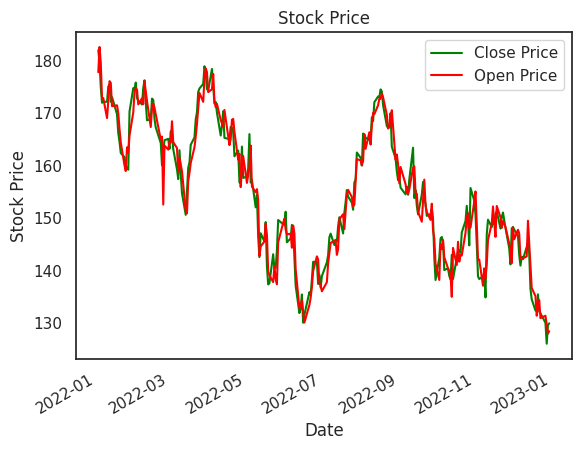
\includegraphics[width=\columnwidth]{stock}
	\caption{The lineplot shows the open and close prices of Apple Inc. stock during 2022.}
	\label{fig:stock}
\end{figure}
This research project delves into the intricate domain of stock price prediction, leveraging an array of advanced machine learning and deep learning methodologies.
Moving beyond the traditional realm of Recurrent Neural Networks (RNNs), the study incorporates a diverse selection of techniques including Gated Recurrent Units (GRU), Long Short-Term Memory networks (LSTM), Transformers, and renowned boosting algorithms like LightGBM, CatBoost, XGBoost, and Random Forest.
Each of these methodologies is selected for its distinct capability in processing and predicting time-series data, which is crucial in the context of financial markets.

A key aspect of this research is the extensive feature engineering process.
This phase involved integrating a comprehensive suite of statistical and financial indicators to form a robust feature set.
These indicators, encompassing historical price trends, volume fluctuations, and market sentiment, were meticulously chosen to ensure a thorough representation of the market dynamics.
Furthermore, the project employed rigorous methods for the combined selection of these features, aiming to maximize the predictive power and efficiency of the models.

The implementation phase of the project was marked by the development of clear, efficient, and well-documented code.
Prioritizing code readability and reusability, along with optimal performance, was fundamental to the success of the experimental procedures.
This meticulous approach allowed for rigorous testing and validation of the various models employed, thereby ensuring the reliability and scholarly integrity of the findings.

Through detailed experimentation, this project goes beyond merely identifying the most effective model for stock price prediction.
It seeks to elucidate the underlying connections between different modeling approaches and feature variables.
Additionally, the study contributes to the theoretical discourse by exploring how these models interact with empirical stock market data.
Ultimately, this research aspires to enrich the academic understanding of stock price prediction and lay down a foundational pathway for future explorations in this evolving field.

\begin{figure}[h]
	\centering
	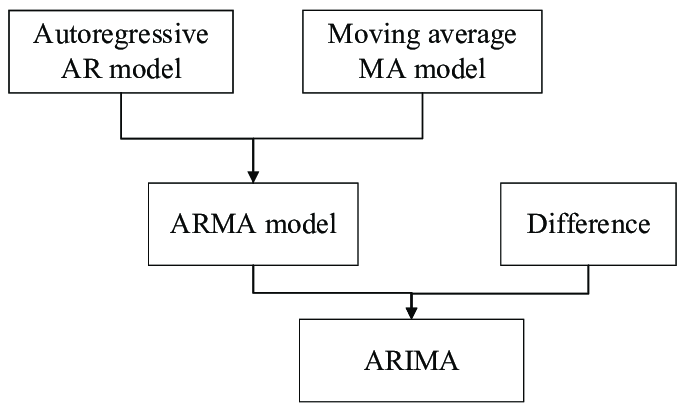
\includegraphics[width=\columnwidth]{arma_arima}
	\caption{The relationship between AR, ARMA and ARIMA.}
	\label{fig:arma_arima}
\end{figure}
\section{Related Work}
\label{sec:related}
\subsection{Auto-Regressive (AR) models}
Autoregressive (AR) models, Autoregressive Moving Average (ARMA) models, and Autoregressive Integrated Moving Average (ARIMA) models\cite{valipour2013comparison, shah2019stock, agrawal2013state}[\ref{fig:arma_arima}] are widely used. Here's a brief overview of each:

The AR model predicts future values based on past values in a time series. The basic idea is that a current observation can be forecasted as a linear combination of past observations. An AR model that uses the past \( p \) values is called an AR($p$) model. Mathematically, an AR($p$) model is expressed as:
\[
	X_t = c + \phi_1 X_{t-1} + \phi_2 X_{t-2} + ... + \phi_p X_{t-p} + \epsilon_t
\]
where \( X_t \) is the current value, \( c \) is a constant, \( \phi_1, \phi_2, ..., \phi_p \) are the model parameters, and \( \epsilon_t \) is white noise.

The ARMA is a combination of the AR model and the Moving Average (MA) model. It includes the autoregressive part of the AR model and adds moving average terms to capture the noise in the time series. An ARMA model is typically denoted as ARMA($p, q$), where \( p \) and \( q \) are the orders of the autoregressive and moving average parts, respectively. An ARMA model is represented as:
\[
	X_t = c + \phi_1 X_{t-1} + ... + \phi_p X_{t-p} + \epsilon_t + \theta_1 \epsilon_{t-1} + ... + \theta_q \epsilon_{t-q}
\]
where \( \theta_1, ..., \theta_q \) are coefficients of the moving average terms.

The ARIMA is an extended form of the ARMA model, used for modeling and forecasting non-stationary time series data. It transforms a non-stationary time series into a stationary one through differencing (calculating the differences between consecutive observations) and then applies an ARMA model. An ARIMA model is usually denoted as ARIMA($p, d, q$), where \( d \) is the degree of differencing. The general form of an ARIMA model is:
\[
	(1 - \phi_1 B - ... - \phi_p B^p)(1 - B)^d X_t = (1 + \theta_1 B + ... + \theta_q B^q) \epsilon_t
\]
where \( B \) is the Backshift Operator, representing the differencing operation.

In stock price prediction, these models are particularly valuable for their ability to capture temporal dependencies and volatility, making them integral tools in financial forecasting.
\subsection{Artificial Neural Networks (ANNs)}
Artificial Neural Networks (ANNs)\cite{shah2019stock,agrawal2013state}[\ref{fig:ann}] have become indispensable in financial market analysis due to their exceptional ability to handle nonlinearity, their data-driven nature, and robust generalization capabilities.
Particularly adept at modeling the complex, interdependent factors in inherently nonlinear financial markets, ANNs excel in capturing and accurately modeling market dynamics, surpassing traditional linear models.
Their data-driven approach is key in analyzing vast volumes of historical market data, allowing them to uncover subtle patterns and trends crucial for prediction.

Moreover, ANNs' ability to generalize from training data ensures their models stay relevant and accurate amidst the constantly evolving market conditions.
This effectiveness is highlighted by their growing adoption for multivariate analysis in finance, where they analyze multiple interrelated variables to understand the combined impact on market behavior.
\begin{figure}[h]
	\centering
	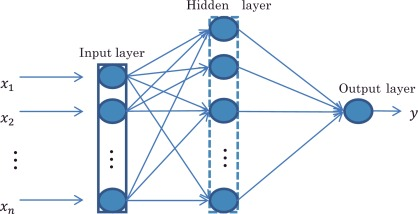
\includegraphics[width=\columnwidth]{ann}
	\caption{Architecture of the three-layered ANN.}
	\label{fig:ann}
\end{figure}
\subsection{Hybrid}
The hybrid approach in the context of stock market prediction involves a strategic combination of various methods to enhance overall performance.
This fusion can take the form of blending statistical and pattern recognition approaches, or integrating statistical techniques with machine learning algorithms.
The goal is to leverage the strengths of each method to create a more robust and accurate predictive model.
Recent research in this field has explored a wide range of algorithms and methods within these categories, seeking to improve the precision and reliability of stock market predictions.

Additionally, the literature has shown a growing interest in hybrid approaches, which incorporate elements from both statistical and machine learning domains.
These hybrid models have been increasingly utilized to tackle the complexities and dynamics of financial markets, aiming to provide more effective tools for investors and analysts to make informed decisions in a volatile and ever-changing environment.

\section{Dataset}
\label{sec:dataset}
The dataset utilized in this study was acquired through the \textit{yahooquery} package, which fetches data from Yahoo Finance. The significance of this dataset lies in its comprehensive capture of daily stock market activities, providing a detailed temporal snapshot of various stock attributes at each time point. Each data entry encompasses the following basic fields[\ref{fig:stock},\ref{tab:aapl}]:
\begin{itemize}
	\item \textbf{Open}: Price at the start of the trading day.
	\item \textbf{High}: Highest price during the trading day.
	\item \textbf{Low}: Lowest price during the trading day.
	\item \textbf{Close}: Price at the end of the trading day.
	\item \textbf{Adjusted Close}: Closing price adjusted for dividends and stock splits.
	\item \textbf{Factor}: Adjustment factor for price changes due to corporate actions.
	\item \textbf{Volume}: Number of shares traded during the day.
\end{itemize}
Additionally, Microsoft's open-source library, \textit{Qlib}\cite{yang2020qlib}, was utilized for further processing of the data. The specifics of these operations will be discussed in subsequent sections.

\begin{table}[t]
	\centering
	\caption{Rounded Apple Inc. Stock Price Data Sample}
	\begin{tabularx}{\columnwidth}{lcccccc}
		\toprule
		Date   & Open & High & Low & Close & Volume & Adj \\
		\midrule
		220103 & 178  & 183  & 178 & 182   & 1.04e8 & 180 \\
		220104 & 183  & 183  & 179 & 180   & 9.93e7 & 178 \\
		220105 & 180  & 180  & 175 & 175   & 9.45e7 & 173 \\
		220106 & 173  & 175  & 172 & 172   & 9.69e7 & 170 \\
		220107 & 173  & 174  & 171 & 172   & 8.67e7 & 170 \\
		\bottomrule
	\end{tabularx}
	\label{tab:aapl}
\end{table}

\section{Problem Statement}
\label{sec:ps}
The primary goal of this research is to develop predictive models for stock prices using time-series data.
This data is characterized by several key features for each stock, each representing crucial aspects of stock performance on a daily basis.
These features are:

Given the time-series nature of this data, the task is to predict future stock prices based on historical data.
The predictions can be approached in several ways:

\begin{enumerate}
	\item \textbf{Direct Feature Prediction}: This involves forecasting the next day's feature values, represented by \( X_{t+1} \), where \( X_{t} \) is an element of the feature vector \( X_{t} \).
	      The mathematical representation for predicting the next day's feature value is as follows:
	      \[
		      X_{t+1} = f(X_t)
	      \]
	      where \( f \) represents the predictive model, and \( X_t \) is the set of features at time \( t \).

	\item \textbf{Predicting Feature Changes}: This method focuses on predicting the change in these features from one day to the next.
	      The change in a particular feature can be represented as:
	      \[
		      \Delta X_{t+1} = X_{t+1} - X_t
	      \]
	      The predictive model aims to estimate \( \Delta X_{t+1} \) based on the feature vector \( X_t \).
\end{enumerate}

Additionally, the models can be extended to predict other aspects such as the High and Low prices or to calculate the expected trading volume for the next day.
The success of these models will be gauged based on their accuracy and reliability in forecasting, which is crucial for effective investment decisions.
The unpredictability and volatility inherent in stock market data present significant challenges, requiring sophisticated modeling techniques and comprehensive feature analysis.
Advanced machine learning and deep learning methods will be employed to analyze the time-series data, and the performance of these models will be rigorously tested against historical data to ensure their effectiveness in real-world scenarios.

%------------------------------------------------------------------------
\section{Methodology}
\label{sec:method}
The methodology of this project is centered around time series forecasting, with a strong emphasis on both theoretical and practical aspects.
The focus is not on implementing various layers and models from scratch but rather on applying these models effectively to predict stock prices.
Given the complexity and dynamic nature of financial markets, the project adopts a comprehensive approach, intertwining advanced forecasting models with effective feature engineering and robust code implementation.
\subsection{Feature Engineering}
\label{sec:fe}
In this project, addressing the challenge of limited original features in stock data is paramount for effective stock price prediction.
Typically, stock datasets consist of basic features are often insufficient for building robust predictive models.
By deriving more technical indicators in feature engineering to enhance the model's predictive power.

Part of selections, as follows:
\begin{itemize}
	\item \textbf{Exponential Moving Average (EMA)}: Gives more weight to recent prices than MA.
	      \begin{align*}
		      s_t & = \alpha x_t + (1 - \alpha) s_{t-1} \\
		          & = s_{t-1} + \alpha (x_t - s_{t-1})
	      \end{align*}
	      where \( \alpha \) is the smoothing factor, and \( 0 \leq \alpha \leq 1 \).

	\item \textbf{Percentage Change (PCT Change)}: Measures the percentage change in price over a period.
	      \begin{align*}
		      \text{PCT Change} = \frac{P_t - P_{t-n}}{P_{t-n}} \times 100
	      \end{align*}
	      where \( P_t \) is the price at time \( t \) and \( P_{t-n} \) is the price \( n \) periods before \( t \).

	\item \textbf{Moving Average Convergence Divergence (MACD)}: Shows the relationship between Difference (DIF) and DEA.
		\begin{align*}
			\text{DIF} &= \text{EMA}_{\text{fast}} - \text{EMA}_{\text{slow}} \\
			\text{DEA} &= \text{EMA}(\text{DIF}, n_{\text{signal}}) \\
			\text{MACD} &= 2 \times (\text{DIF} - \text{DEA})
		\end{align*}
		where \( \text{EMA}_{\text{fast}} \) and \( \text{EMA}_{\text{slow}} \) are fast and slow EMAs, respectively. \( n_{\text{signal}} \) is typically 9 periods.

	\item \textbf{Skewness}: Measures asymmetry of the distribution of returns.
	      \begin{align*}
		      \text{Skewness} = \frac{E[(X-\mu)^3]}{\sigma^3}
	      \end{align*}
	      where \( X \) is a random variable, \( E \) is the expected value, \( \mu \) is the mean, and \( \sigma \) is the standard deviation.

	\item \textbf{Kurtosis}: Measures the "tailedness" of the return distribution.
	      \begin{align*}
		      \text{Kurtosis} = \frac{E[(X-\mu)^4]}{\sigma^4}
	      \end{align*}
	      where \( X \), \( E \), \( \mu \), and \( \sigma \) are as defined in Skewness.

	\item \textbf{Mean Absolute Deviation (MAD)}: The average of the absolute deviations from a central point.
	      \begin{align*}
		      \text{MAD} = \frac{\sum_{i=1}^{n} |X_i - \bar{X}|}{n}
	      \end{align*}
	      where \( X_i \) are individual observations and \( \bar{X} \) is the mean.

	\item \textbf{Momentum}: Measures the rate of change in prices.
	      \begin{align*}
		      \text{Momentum} = P_t - P_{t-n}
	      \end{align*}
	      where \( P_t \) is the price at time \( t \) and \( P_{t-n} \) is the price \( n \) periods before \( t \).

	\item \textbf{Relative Strength Index (RSI)}: Measures recent price changes to assess overbought or oversold conditions.
	      \begin{align*}
		      \text{RSI} = 100 - \frac{100}{1 + \text{RS}}
	      \end{align*}
	      where \( \text{RS} \) is the average gain divided by the average loss.

	\item \textbf{Bollinger Bands}: Consist of an MA (middle band) and two standard deviation lines.
	      \begin{align*}
		      \text{Upper Band} = \text{MA} + 2 \times \text{SD} \\
		      \text{Lower Band} = \text{MA} - 2 \times \text{SD}
	      \end{align*}
	      where \( \text{SD} \) is the standard deviation.

	\item \textbf{Average Directional Index (ADX)}: Measures the strength of a trend.

	\item \textbf{Directional Movement Index (DMI)}: Includes Positive Direction ($+DI$) and Negative Direction ($-DI$) indicators to measure the direction of price movement.
\end{itemize}
Most methods are choosed from \textit{101 Formulaic Alphas}\cite{zura2015101} some are implemented using the built-in expression in \textit{Qlib}\cite{yang2020qlib}, and the rest are implemented using \textit{numpy} and \textit{pandas}.
\begin{figure}[t]
	\centering
	\subfloat[]{\label{fig:raw_corr}\includegraphics[width=0.5\columnwidth]{raw_feats}}
	\subfloat[]{\label{fig:sel}\includegraphics[width=0.5\columnwidth]{sel_feats}}
	\caption{The left image shows the correlation matrix after detailed and comprehensive feature engineering, while the right image displays the correlation matrix after feature selection.}
	\label{fig:feat_corr}
\end{figure}
\subsection{Feature Selection}
\label{sec:fs}
In stock price prediction, the significance of feature selection following feature engineering is crucial.
Developing a comprehensive set of features is essential, but more importantly, selecting the most impactful ones is key.
This process streamlines the model, enhancing predictive accuracy and avoiding overfitting.
The correlation matrix[\ref{fig:feat_corr}] plays a critical role in this stage by shedding light on the relationships among features, especially in identifying and avoiding multicollinearity, which can skew model results.
Appropriate feature selection methods are vital to reducing complexity and ensuring a robust and efficient model, adept at making reliable predictions in the volatile stock market environment.

\textbf{Statistical Test-Based Selection}: Applying a variety of statistical tests, including Chi-square test, Pearson's correlation, F-test, and mutual information methods.
These tests are selected to capture different types of relationships between features and stock prices: Chi-square for categorical relations, Pearson's correlation and the F-test for linear relationships, and mutual information for nonlinear dependencies\cite{pedregosa2011scikit}.
The top 50 features from each test are selected, ensuring a comprehensive yet manageable feature set.

\textbf{Recursive Feature Elimination (RFE)}: Using RFE with Linear Regression, methodically refines the feature set.
By iteratively removing less impactful features, it concentrates on those most predictive in a linear context, simplifying the model while retaining crucial linear predictive elements\cite{pedregosa2011scikit}.

\textbf{Model-Based Selection}: Utilizing a RandomForestRegressor in conjunction with SelectFromModel targets more complex patterns.
This approach is adept at identifying nonlinear interactions within the data, key to accurately modeling the nuanced dynamics of stock markets.

\subsection{Recurrent Neural Network (RNN)}
\label{sec:rnns}
RNNs have emerged to efficiently handle sequential data by overcoming the limitations of traditional neural networks, which excel with static data but struggle with time-series data due to their inability to capture temporal sequence information\cite{rumelhart1986learning}.
RNNs incorporate loop structures within the network, facilitating the retention and utilization of historical data across different time steps. Consequently, RNNs are well-suited for tasks where output depends on previous information.

\subsubsection{Vanilla}
\label{sec:vani}
RNNs are designed to process sequential data by using their internal state (memory) to capture information about previous elements in the sequence, making them suitable for tasks like time series prediction or language modeling.

The RNN structure[\ref{fig:rnn}] involves a simple loop where the hidden state from the previous timestep is combined with the current input to produce the current hidden state, which is then used for predictions or passed to the next timestep.

Mathematically, a RNN can be represented as:
\begin{align*}
	\mathbf{H}_t &= \phi(\mathbf{X}_t \mathbf{W}_{\textrm{xh}} + \mathbf{H}_{t-1} \mathbf{W}_{\textrm{hh}}  + \mathbf{b}_\textrm{h}), \\
	\mathbf{O}_t &= \mathbf{H}_t \mathbf{W}_{\textrm{hq}} + \mathbf{b}_\textrm{q},
\end{align*}
where \( \mathbf{H}_t \) is the hidden state at time \( t \), \( \phi \) is an activation function (often tanh or ReLU), \( \mathbf{X}_t \) is the input at time \( t \), \( \mathbf{W}_{\textrm{xh}} \) and \( \mathbf{W}_{\textrm{hh}} \) are weight matrices, \( \mathbf{b}_\textrm{h} \) is the bias for the hidden layer, and \( \mathbf{O}_t \) is the output at time \( t \).
\begin{figure}[h]
	\centering
	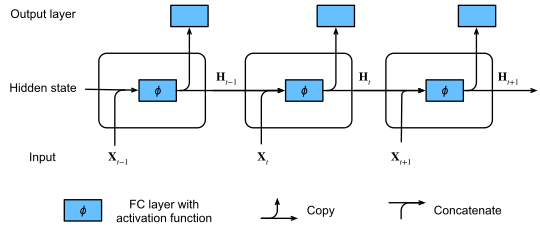
\includegraphics[width=\columnwidth]{rnn}
	\caption{An RNN with a hidden state\cite{zhang2023dive}.}
	\label{fig:rnn}
\end{figure}
\textbf{Backpropagation Through Time (BPTT)} is an algorithm for training Recurrent Neural Networks (RNNs). It involves:
\begin{enumerate}
    \item Unrolling the RNN across time steps.
    \item Performing a forward pass to compute outputs.
    \item Calculating gradients during a backward pass from output to input.
    \item Updating weights based on these gradients.
\end{enumerate}
Challenges include vanishing and exploding gradients\cite{rumelhart1986learning}.
\subsubsection{Long Short-Term Memory (LSTM)}
\label{sec:lstm}
LSTMs further enhance the ability to capture long-term dependencies in sequential data through a more sophisticated architecture involving a cell state and three types of gates (input, output, and forget gates)\cite{memory2010long, yu2019review}[\ref{fig:lstm}], providing a more nuanced control over the memory component of the network.

LSTMs consist of a cell state running through the chain, with gates controlling the state's information flow. The cell state carries long-term information, while the gates regulate the information added to or removed from the cell state, as well as the information passed to the output.

Mathematically, an LSTM can be represented as:
\begin{align*}
	\mathbf{I}_t &= \sigma(\mathbf{X}_t \mathbf{W}_{\textrm{xi}} + \mathbf{H}_{t-1} \mathbf{W}_{\textrm{hi}} + \mathbf{b}_\textrm{i}),\\
	\mathbf{F}_t &= \sigma(\mathbf{X}_t \mathbf{W}_{\textrm{xf}} + \mathbf{H}_{t-1} \mathbf{W}_{\textrm{hf}} + \mathbf{b}_\textrm{f}),\\
	\mathbf{O}_t &= \sigma(\mathbf{X}_t \mathbf{W}_{\textrm{xo}} + \mathbf{H}_{t-1} \mathbf{W}_{\textrm{ho}} + \mathbf{b}_\textrm{o}), \\
	\tilde{\mathbf{C}}_t &= \textrm{tanh}(\mathbf{X}_t \mathbf{W}_{\textrm{xc}} + \mathbf{H}_{t-1} \mathbf{W}_{\textrm{hc}} + \mathbf{b}_\textrm{c}),\\
	\mathbf{C}_t &= \mathbf{F}_t \odot \mathbf{C}_{t-1} + \mathbf{I}_t \odot \tilde{\mathbf{C}}_t,\\
	\mathbf{H}_t &= \mathbf{O}_t \odot \tanh(\mathbf{C}_t),
\end{align*}
where \( \sigma \) is the sigmoid function, \( \mathbf{I}_t, \mathbf{F}_t, \mathbf{O}_t \) are the input, forget, and output gates, respectively, \( \mathbf{C}_t \) is the cell state, and \( \mathbf{H}_t \) is the hidden state.  \( \odot \) represents Hadamard product operator.
\begin{figure}[h]
	\centering
	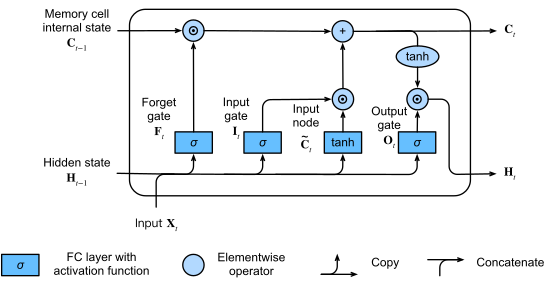
\includegraphics[width=\columnwidth]{lstm}
	\caption{Computing the hidden state in an LSTM model\cite{zhang2023dive}.}
	\label{fig:lstm}
\end{figure}
\subsubsection{Gated Recurrent Unit (GRU)}
\label{sec:gru}
GRUs improve upon RNNs by introducing gates (update and reset gates) that help in managing the flow of information and addressing the vanishing gradient problem\cite{cho2014learning}[\ref{fig:gru}], thus making them more effective in capturing long-range dependencies within the sequence.

GRUs simplify the LSTM structure by merging the cell state and hidden state and using two gates. These gates control the flow of information inside the unit, deciding what to keep from the past and what new information to add.

Mathematically, a GRU can be represented as:
\begin{align*}
	\mathbf{R}_t &= \sigma(\mathbf{X}_t \mathbf{W}_{\textrm{xr}} + \mathbf{H}_{t-1} \mathbf{W}_{\textrm{hr}} + \mathbf{b}_\textrm{r}),\\
	\mathbf{Z}_t &= \sigma(\mathbf{X}_t \mathbf{W}_{\textrm{xz}} + \mathbf{H}_{t-1} \mathbf{W}_{\textrm{hz}} + \mathbf{b}_\textrm{z}),	\\
	\tilde{\mathbf{H}}_t &= \tanh(\mathbf{X}_t \mathbf{W}_{\textrm{xh}} + \left(\mathbf{R}_t \odot \mathbf{H}_{t-1}\right) \mathbf{W}_{\textrm{hh}} + \mathbf{b}_\textrm{h}),\\
	\mathbf{H}_t &= \mathbf{Z}_t \odot \mathbf{H}_{t-1}  + (1 - \mathbf{Z}_t) \odot \tilde{\mathbf{H}}_t.	
\end{align*}
where \( \mathbf{R}_t \) and \( \mathbf{Z}_t \) are the reset and update gates, respectively, \( \mathbf{H}_t \) is the hidden state, and \( \tilde{\mathbf{H}}_t \) is the candidate hidden state. \( \odot \) represents Hadamard product operator.
\begin{figure}[h]
	\centering
	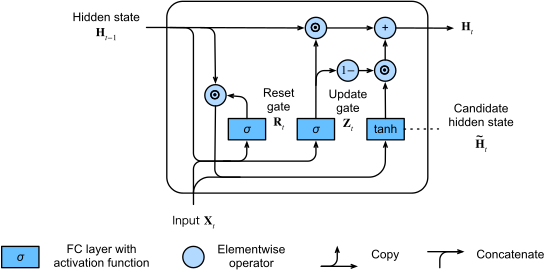
\includegraphics[width=\columnwidth]{gru}
	\caption{Computing the hidden state in a GRU model\cite{zhang2023dive}.}
	\label{fig:gru}
\end{figure}
\subsubsection{Deep Recurrent Neural Networks}
\label{sec:drnn}
Deep Recurrent Neural Networks (DRNNs) are an extension of basic RNNs that include multiple hidden layers at each time step\cite{pascanu2019construct}. This architecture[\ref{fig:drnn}] allows the network to capture more complex features and relationships in the data.

In a DRNN, each layer's hidden state not only depends on the previous time step's state of the same layer but also receives input from the hidden state of the previous layer at the same time step.

Mathematically, a DRNN with \( L \) layers can be represented as:
\begin{align*}
	\mathbf{H}_t^{(l)} &= \phi_l(\mathbf{H}_t^{(l-1)} \mathbf{W}_{\textrm{xh}}^{(l)} + \mathbf{H}_{t-1}^{(l)} \mathbf{W}_{\textrm{hh}}^{(l)}  + \mathbf{b}_\textrm{h}^{(l)}),\\
	\mathbf{O}_t &= \mathbf{H}_t^{(L)} \mathbf{W}_{\textrm{hq}} + \mathbf{b}_\textrm{q},
\end{align*}
where \( \mathbf{H}_t^{(l)} \) is the hidden state of the \( l \)-th layer at time \( t \), \( \phi_l \) is an activation function for layer \( l \), \( \mathbf{W}_{\textrm{xh}}^{(l)} \) and \( \mathbf{W}_{\textrm{hh}}^{(l)} \) are weight matrices, and \( \mathbf{b}_\textrm{h}^{(l)} \) is the bias for layer \( l \).
\begin{figure}[h]
	\centering
	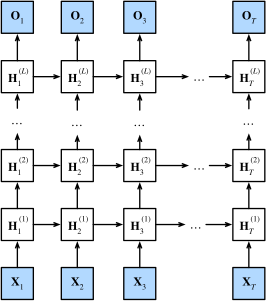
\includegraphics[width=0.7\columnwidth]{deep-rnn}
	\caption{Architecture of a deep RNN\cite{zhang2023dive}.}
	\label{fig:drnn}
\end{figure}
\subsubsection{Bidirectional Recurrent Neural Networks}
\label{sec:birnn}
Bidirectional Recurrent Neural Networks (BiRNNs) process data in both forward and backward directions. This approach allows the network to have both past and future context, improving its ability to understand the sequence\cite{schuster1997bidirectional}.

In a BiRNN, two separate hidden layers process the sequence in opposite directions[\ref{fig:brnn}]. The outputs of these two layers are typically combined at each time step, either by summing, concatenating, or another method.

Mathematically, a BiRNN can be represented as:
\begin{align*}
	\overrightarrow{\mathbf{H}}_t &= \phi(\mathbf{X}_t \mathbf{W}_{\textrm{xh}}^{(f)} + \overrightarrow{\mathbf{H}}_{t-1} \mathbf{W}_{\textrm{hh}}^{(f)}  + \mathbf{b}_\textrm{h}^{(f)}),\\
	\overleftarrow{\mathbf{H}}_t &= \phi(\mathbf{X}_t \mathbf{W}_{\textrm{xh}}^{(b)} + \overleftarrow{\mathbf{H}}_{t+1} \mathbf{W}_{\textrm{hh}}^{(b)}  + \mathbf{b}_\textrm{h}^{(b)}),\\
	\mathbf{O}_t &= \mathbf{H}_t \mathbf{W}_{\textrm{hq}} + \mathbf{b}_\textrm{q}.
\end{align*}
where \( \overrightarrow{\mathbf{H}}_t \) and \( \overleftarrow{\mathbf{H}}_t \) are the forward and backward hidden states at time \( t \), respectively.
\begin{figure}[h]
	\centering
	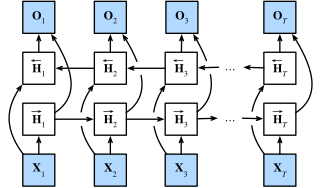
\includegraphics[width=0.7\columnwidth]{birnn}
	\caption{Architecture of a bidirectional RNN\cite{zhang2023dive}.}
	\label{fig:brnn}
\end{figure}
\subsection{Transformer}
\label{sec:transformer}
Transformers represent a significant shift in neural network architecture, particularly for natural language processing tasks.
Unlike previous models reliant on sequential processing (like RNNs and LSTMs), Transformers use a mechanism called attention to process entire sequences of data in parallel.
This architecture has led to substantial improvements in various tasks like machine translation, text generation, and more.
\subsubsection{Attention Mechanism}
\label{sec:attention}
The Attention Mechanism\cite{vaswani2017attention} is a critical component of the Transformer architecture. It allows the model to dynamically focus on different parts of the input sequence, determining which parts are most relevant for a given task.

Mathematically, the attention can be represented as:
\begin{align*}
    \text{Attention}(Q, K, V) &= \text{softmax}\left(\frac{QK^T}{\sqrt{d_k}}\right)V,
\end{align*}
where \( Q, K, V \) are the query, key, and value matrices, respectively, and \( d_k \) is the dimension of the key.
\subsubsection{Multi-Head Attention}
\label{sec:multi-head}
Multi-Head Attention\cite{vaswani2017attention} allows the Transformer to process information through multiple attention mechanisms in parallel[\ref{fig:mha}]. This approach enables the model to capture different types of relationships in the data.

The Multi-Head Attention is defined as:
\begin{align*}
    \text{MultiHead}(Q, K, V) &= \text{Concat}(\text{head}_1, \ldots, \text{head}_h)W^O, \\
    \text{where head}_i &= \text{Attention}(QW^Q_i, KW^K_i, VW^V_i),
\end{align*}
where \( W^Q_i, W^K_i, W^V_i, \) and \( W^O \) are parameter matrices.
\begin{figure}[h]
	\centering
	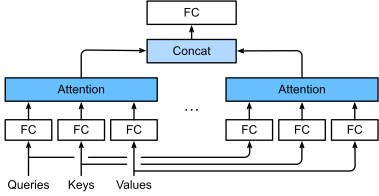
\includegraphics[width=\columnwidth]{mha}
	\caption{Multi-head attention, where multiple heads are concatenated then linearly transformed\cite{zhang2023dive}.}
	\label{fig:mha}
\end{figure}
\subsubsection{Self-Attention}
\label{sec:self-attention}
Self-Attention\cite{vaswani2017attention}, a variant of the attention mechanism, allows each position in the sequence to attend to all positions within the same layer. This enables the model to understand the context and relationships within the sequence itself.

Mathematically, Self-Attention is expressed as:
\begin{align*}
    \text{SelfAttention}(Q, K, V) &= \text{Attention}(Q, K, V),
\end{align*}
where \( Q, K, V \) are all derived from the same input.
\subsubsection{Transformer Block}
\label{sec:transformer-block}
A Transformer block is the fundamental building block of a Transformer model. Each block consists of two main components: a Multi-Head Attention layer and a position-wise Feed-Forward Neural Network\cite{vaswani2017attention}. The attention layer enables the block to focus on different parts of the input sequence, while the feed-forward network processes the sequence in a position-wise manner. Layer Normalization and residual connections are also typically used around each of these components to improve training stability and performance.
\begin{figure}[h]
	\centering
	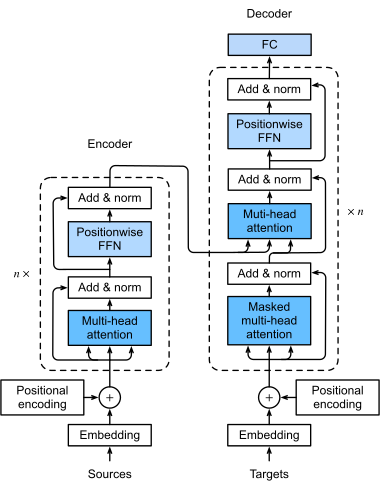
\includegraphics[width=0.7\columnwidth]{transformer}
	\caption{The Transformer architecture. Left and right boxes are 1 encoder block and decoder respectively\cite{zhang2023dive}.}
	\label{fig:trans}
\end{figure}
\subsubsection{Transformer Encoder-Decoder}
\label{sec:transformer-enc-dec}
The Transformer model is structured into two main components: the encoder and the decoder[\ref{fig:trans}]. Each encoder and decoder in the Transformer comprises multiple layers of Transformer blocks, allowing the model to capture complex dependencies and relationships in the data\cite{vaswani2017attention}. This architecture enables the model to effectively handle a wide range of sequence-to-sequence tasks, such as machine translation, by efficiently processing large sequences in parallel while capturing intricate relationships within the data.

\subsection{Boosting}
\label{sec:bst}
The decision to use LightGBM, XGBoost, and CatBoost\cite{chen2016xgboost, prokhorenkova2018catboost, ke2017lightgbm} in stock price prediction is motivated by personal interest and a desire to explore their applicability.
These boosting algorithms are known for their efficiency, accuracy, and suitability for complex datasets.
Applying them to stock prediction allows for an in-depth investigation of their mechanics and real-world performance in finance.
This exploration aids in understanding their strengths, limitations, and adaptability across scenarios, including challenging financial time series analysis. Although not designed for time series tasks, I aim to assess their ability to capture temporal relationships in data through extensive feature engineering.

\section{Losses and Metrics}
\label{sec:le}
\textbf{Mean Squared Error (MSE)}: The average of the squares of the errors, being more sensitive to large errors. It is commonly used for regression tasks.
\begin{equation}
    \text{MSE} = \frac{1}{n} \sum_{i=1}^{n} (Y_i - \hat{Y}_i)^2
\end{equation}

\textbf{Root Mean Squared Error (RMSE)}: The square root of MSE, providing error in the same units as the data. It is sensitive to large errors but less so than MSE.
\begin{equation}
    \text{RMSE} = \sqrt{\frac{1}{n} \sum_{i=1}^{n} (Y_i - \hat{Y}_i)^2}
\end{equation}

\textbf{Mean Absolute Error (MAE)}: The average of the absolute differences between predicted and actual values, offering stable error metrics with less sensitivity to outliers.
\begin{equation}
    \text{MAE} = \frac{1}{n} \sum_{i=1}^{n} |Y_i - \hat{Y}_i|
\end{equation}

\textbf{Mean Absolute Percentage Error (MAPE)}: The average absolute percent error between the predicted and actual values. It's easily interpretable but unstable for values near or equal to zero.
\begin{equation}
    \text{MAPE} = \frac{1}{n} \sum_{i=1}^{n} \left|\frac{Y_i - \hat{Y}_i}{Y_i}\right| \times 100\%
\end{equation}

\textbf{Root Mean Squared Logarithmic Error (RMSLE)}: The differences between the log-transformed predicted and actual values, being sensitive to small errors and suitable for non-negative numbers with small differences.
\begin{equation}
    \text{RMSLE} = \sqrt{\frac{1}{n} \sum_{i=1}^{n} (\log(Y_i + 1) - \log(\hat{Y}_i + 1))^2}
\end{equation}

\textbf{R-squared (R²)}: The degree of variation in the outcome explained by the model, with values closer to 1 indicating better model fit.
\begin{equation}
    R^2 = 1 - \frac{\sum_{i=1}^{n} (Y_i - \hat{Y}_i)^2}{\sum_{i=1}^{n} (Y_i - \bar{Y})^2}
\end{equation}

\textbf{Differences:}
\begin{itemize}
    \item \textbf{Sensitivity to Outliers}: MSE and RMSE are more sensitive to large errors due to the squaring of errors. In contrast, MAE is less influenced by outliers as it considers absolute differences.
    \item \textbf{Error Units}: MSE and RMSE have different units from the original data (squared and root units respectively), whereas MAE maintains the same units as the original data.
    \item \textbf{Relative vs Absolute Error}: MAPE focuses on relative errors, making it more interpretable in terms of percentage differences. MSE, RMSE, and MAE provide absolute error measures.
    \item \textbf{Sensitivity to Small Errors}: RMSLE is sensitive to small errors by applying a logarithmic scale, making it suitable for cases where the predicted and actual values are both positive and have small differences.
    \item \textbf{Model Fit}: R² is a measure of how well the model fits the data, rather than a direct measure of error. A higher R² value indicates a better fit.
\end{itemize}

%------------------------------------------------------------------------
\begin{table*}[htbp]
	\centering
	\caption{Adjusted close price and residual price Table (rounded in 2 decimals).}
	\adjustbox{max width=\textwidth}{
	\begin{tabular}{l
		*{30}{@{}S[table-format=1.5, round-mode=places, round-precision=2]@{}}} % Adjust the number of columns accordingly
	  \toprule
	  & \multicolumn{18}{c}{Close} & \multicolumn{12}{c}{Delta} \\
	  \cmidrule(lr){2-19} \cmidrule(lr){20-31}
	  & \multicolumn{6}{c}{Basic} & \multicolumn{6}{c}{Full Feature} & \multicolumn{6}{c}{Selected} & \multicolumn{4}{c}{Basic} & \multicolumn{4}{c}{Full Feature} & \multicolumn{4}{c}{Selected} \\
	  \cmidrule(lr){2-7} \cmidrule(lr){8-13} \cmidrule(lr){14-19} \cmidrule(lr){20-23} \cmidrule(lr){24-27} \cmidrule(lr){28-31}
	  & {MSE} & {RMSE} & {MAE} & {MAPE} & {RMSLE} & {R2} & {MSE} & {RMSE} & {MAE} & {MAPE} & {RMSLE} & {R2} & {MSE} & {RMSE} & {MAE} & {MAPE} & {RMSLE} & {R2} & {RMSE} & {MAE} & {MAPE} & {R2} & {RMSE} & {MAE} & {MAPE} & {R2} & {RMSE} & {MAE} & {MAPE} & {R2} \\
	  \midrule
	  RNN & 0.67 & 0.82 & 0.70 & 0.28 & 0.26 & -0.75 & 0.30 & 0.55 & 0.44 & 0.17 & 0.16 & 0.22 & 0.76 & 0.87 & 0.76 & 0.30 & 0.28 & -0.99 & 0.42 & 0.31 & 2.95 & -0.05 & 0.42 & 0.30 & 2.94 & -0.02 & 0.41 & 0.30 & 2.86 & -0.01 \\
	  LSTM & 0.12 & 0.34 & 0.28 & 0.11 & 0.10 & 0.69 & 0.96 & 0.98 & 0.85 & 0.34 & 0.32 & -1.49 & 1.46 & 1.21 & 1.07 & 0.43 & 0.42 & -2.80 & 0.41 & 0.30 & 2.96 & -0.00 & 0.41 & 0.30 & 2.95 & -0.00 & 0.41 & 0.30 & 2.96 & 0.00 \\
	  GRU & 0.10 & 0.32 & 0.26 & 0.10 & 0.09 & 0.73 & 0.82 & 0.91 & 0.79 & 0.32 & 0.29 & -1.14 & 0.60 & 0.78 & 0.68 & 0.27 & 0.25 & -0.57 & 0.41 & 0.30 & 2.88 & 0.00 & 0.41 & 0.30 & 2.97 & -0.00 & 0.41 & 0.30 & 2.93 & 0.00 \\
	  BiGRU & 0.31 & 0.56 & 0.48 & 0.19 & 0.17 & 0.19 & 1.15 & 1.07 & 0.95 & 0.39 & 0.36 & -1.99 & 0.72 & 0.85 & 0.73 & 0.30 & 0.27 & -0.87 & 0.41 & 0.30 & 2.94 & 0.00 & 0.41 & 0.29 & 2.92 & 0.00 & 0.41 & 0.30 & 2.90 & -0.00 \\
	  Transformer & 2.24 & 1.50 & 1.38 & 0.59 & 0.57 & -4.82 & 0.05 & 0.23 & 0.18 & 0.09 & 0.07 & 0.86 & 0.19 & 0.44 & 0.36 & 0.15 & 0.13 & 0.50 & 0.41 & 0.30 & 3.00 & 0.00 & 0.41 & 0.30 & 3.01 & 0.00 & 0.41 & 0.30 & 3.00 & -0.00 \\
	  \bottomrule
	\end{tabular}
	}
	\label{table:met}
\end{table*}	
\section{Experiments}
\label{sec:exper}
Through comprehensively testing various combinations and configurations, and by carefully observing and analyzing the experimental results, individuals can delve deeper into understanding the strengths, weaknesses, and nuances of different techniques. This iterative process of exploration and reflection not only helps in evaluating the effectiveness and applicability of these techniques in different contexts but also fosters a deeper comprehension of the underlying principles and mechanics
\subsection{Experiments Environment}
\label{exper:env}
The experimental platform consists of an AMD 7950X with 16 cores, 64GB RAM, and an NVIDIA RTX4090 with 24GB VRAM. The versions of PyTorch used are 2.1.1, with a CUDA version of 12.1.
\subsection{Experimental Results}
\label{exper:env_res}
All the experiments are the average results after multiple iterations.
\begin{figure}[h]
	\centering
	\subfloat[]{\label{fig:bstv}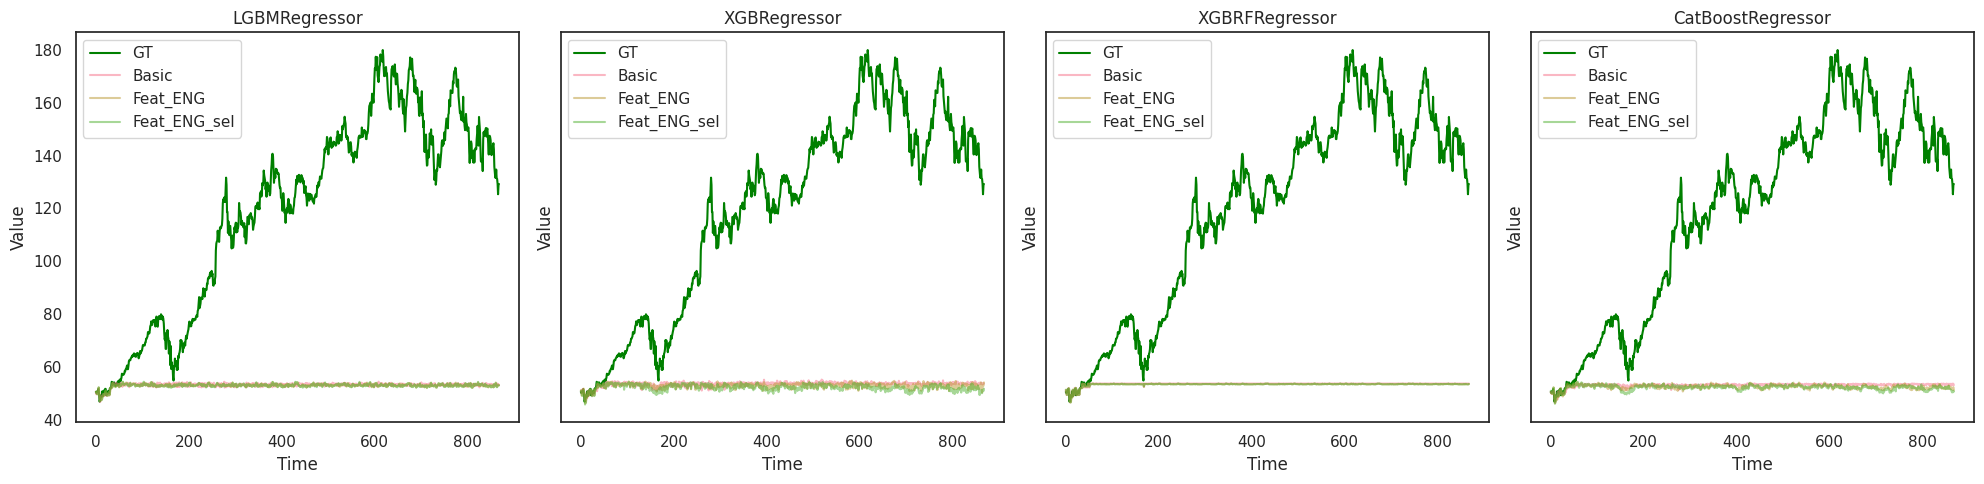
\includegraphics[width=\columnwidth]{boost_value}} \\
	\subfloat[]{\label{fig:bstd}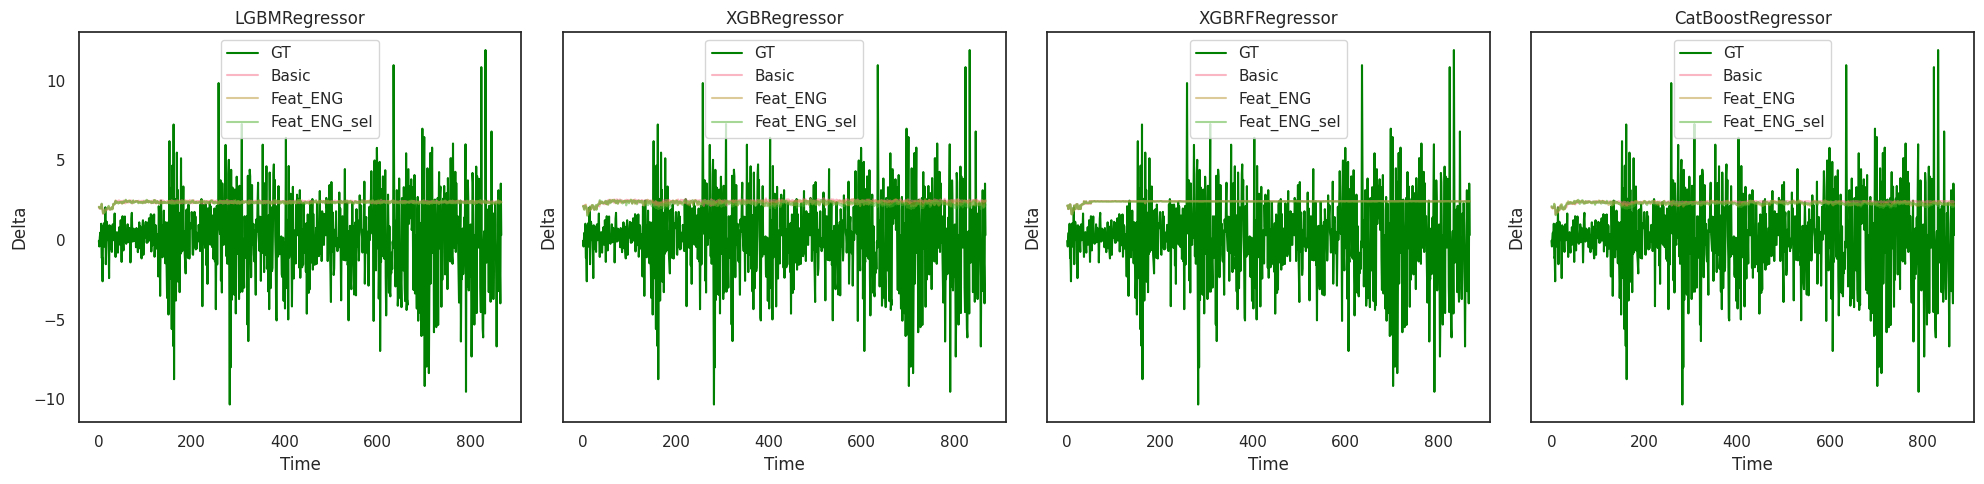
\includegraphics[width=\columnwidth]{boost_delta}}
	\caption{The upper plots show closing prices and lower plots show residual prices in boosting method.}
	\label{fig:bst_res}
\end{figure}

I initially conducted experiments using boosting methods, employing three different sets of features. I performed regression on both closing prices and price residuals[\ref{fig:bst_res}].
For LightGBM, XGBoost, and CatBoost, I utilized their respective Regressors to perform regression based on the input features.
Additionally, I also utilized the Random Forest Regressor from XGBoost. Since these experiments were exploratory in nature, all parameters were kept at their default settings.
\begin{figure}[h]
	\centering
	\subfloat[]{\label{fig:rmc}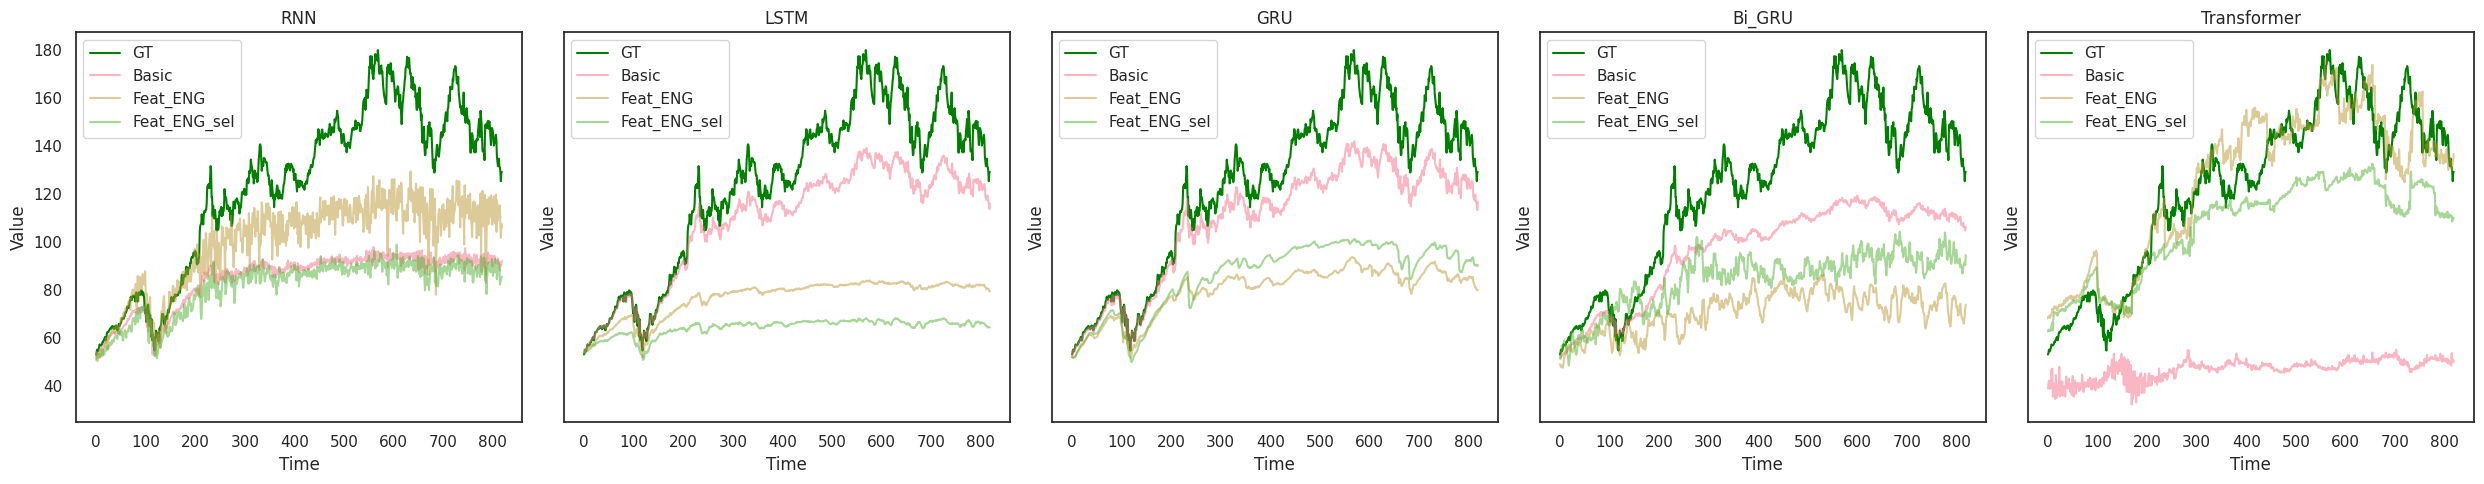
\includegraphics[width=\columnwidth]{res_model_cls}} \\
	\subfloat[]{\label{fig:rmd}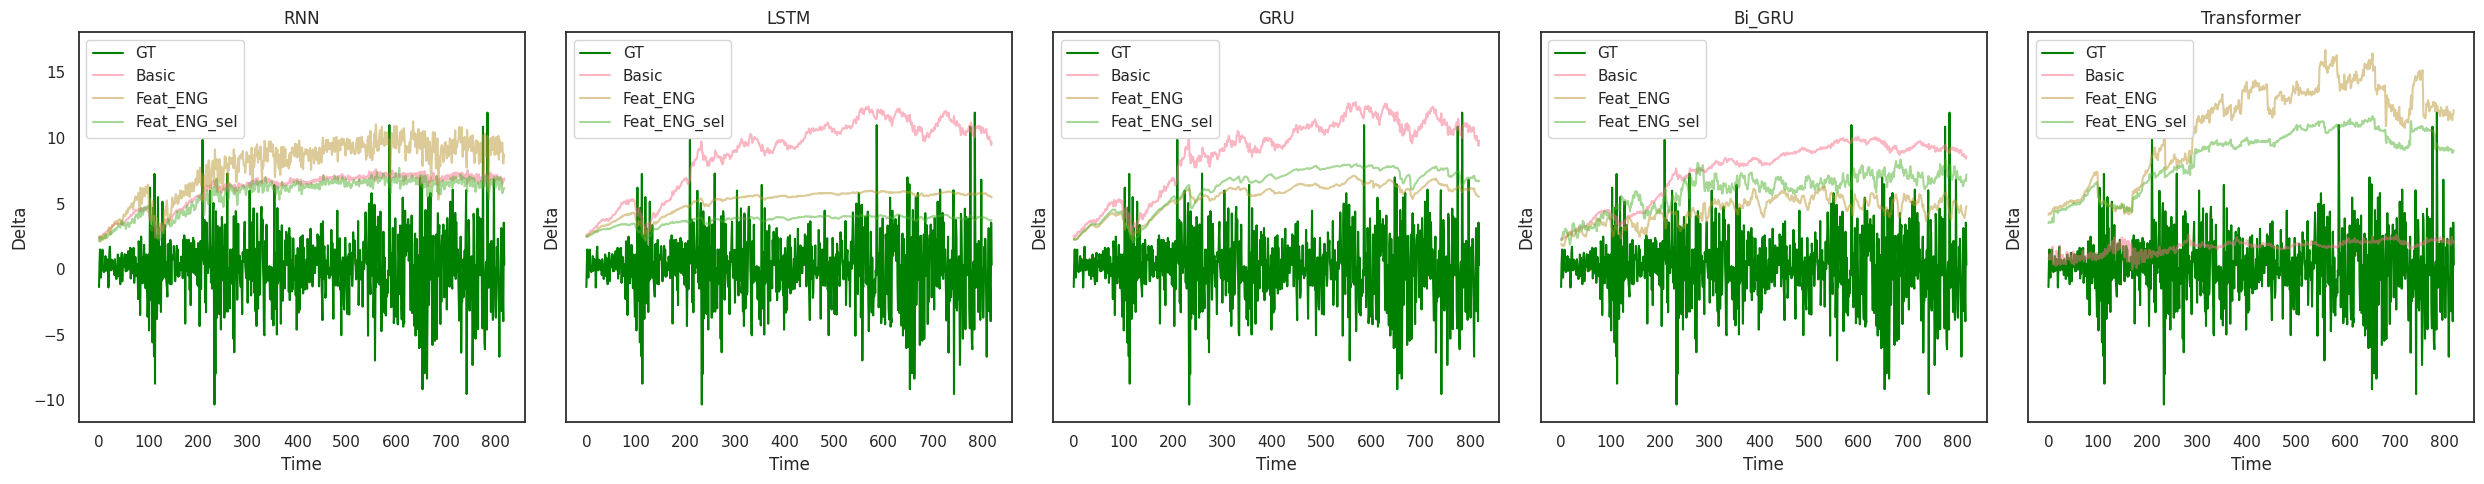
\includegraphics[width=\columnwidth]{res_model_dlt}}
	\caption{The performance of different models in different feature engineering levels.}
	\label{fig:model_res}
\end{figure}

For all RNN-based models, I defaulted to using deep RNNs with 2 layers. The Transformer has 4 attention heads and 2 layers because it's not a sequence-to-sequence model; I only utilized the Transformer Encoder. Two separate charts were created, each corresponding to different model performances under the same set of features[\ref{fig:feats_res}] and different feature performances under the same model[\ref{fig:model_res}].
\begin{figure}[h]
	\centering
	\subfloat[]{\label{fig:rfc}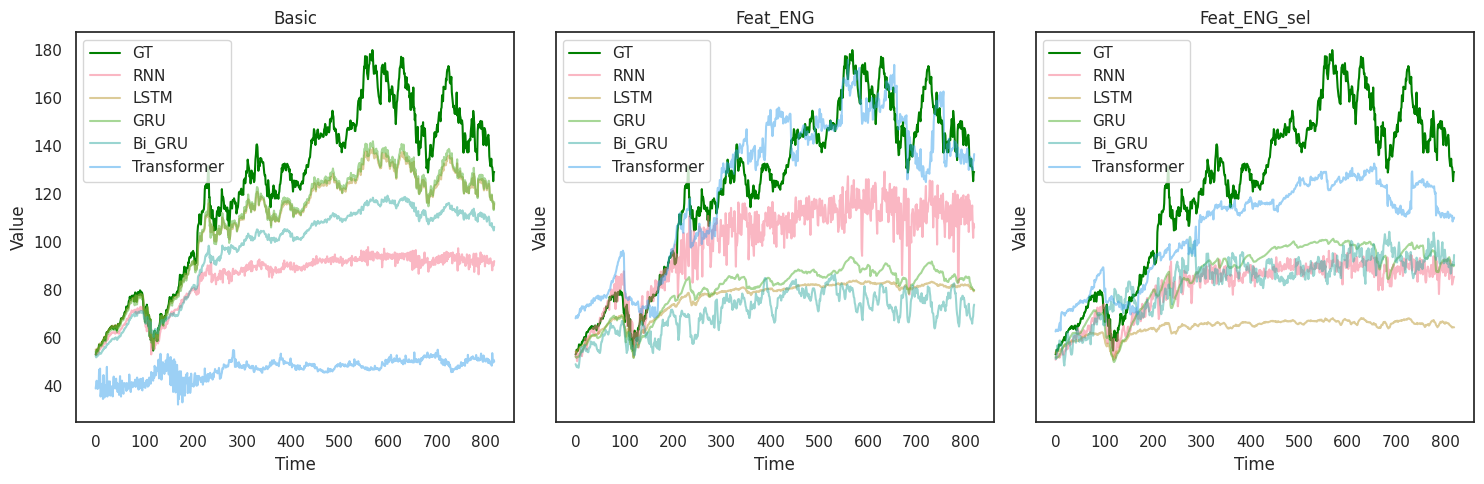
\includegraphics[width=\columnwidth]{res_feat_cls}} \\
	\subfloat[]{\label{fig:rfd}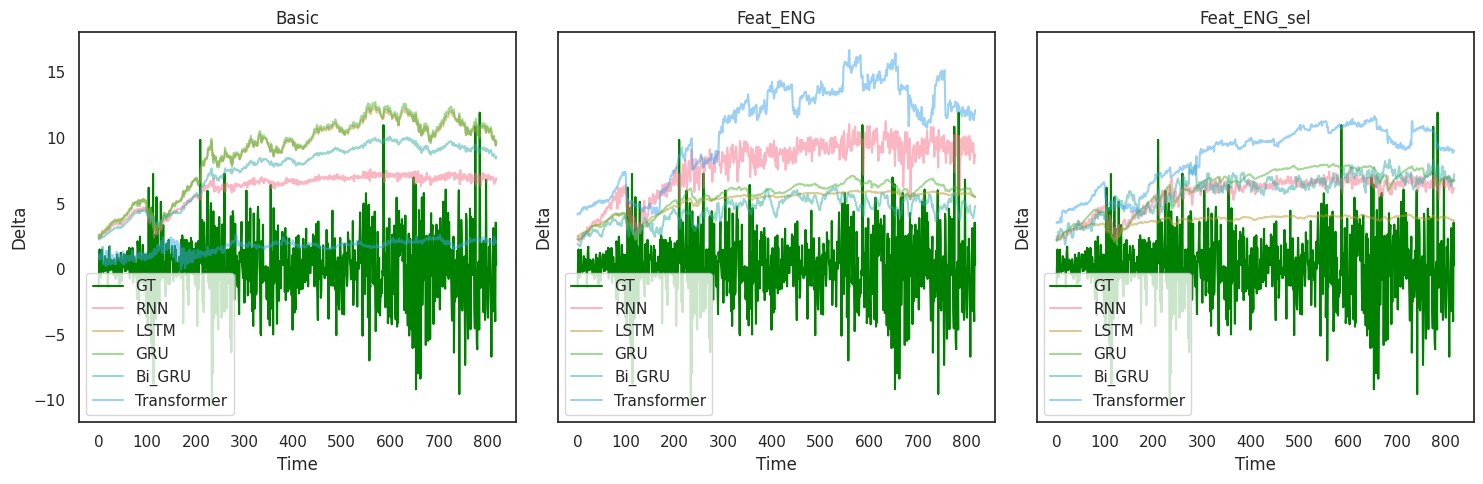
\includegraphics[width=\columnwidth]{res_feat_dlt}}
	\caption{The performance of different feature engineering levels in different models.}
	\label{fig:feats_res}
\end{figure}

There is a table of metrics, corresponding to closing prices and price residuals under different models and features[\ref{table:met}]. Since the range of price residuals includes both positive and negative values, some metrics cannot be used.
\section{Analysis of Feature and Model Performance}
\label{sec:ra}

\begin{itemize}
    \item \textbf{RNN}: On low-dimensional basic features, RNN performs moderately, likely due to its limited ability to handle complex time series dependencies. After introducing financial indicators, performance improved, suggesting RNN benefits from the increased information. However, after feature selection, performance slightly declined, possibly indicating that the selected features do not fully align with the RNN model's optimization path.
    
    \item \textbf{LSTM}: For basic feature sets, LSTM demonstrates its ability to capture long-term dependencies, but performance declined after the introduction of complex financial indicators, likely due to the complexity exceeding LSTM's processing capacity. Performance recovered after feature selection, suggesting that the filtered features are more suitable for the LSTM model.
    
    \item \textbf{GRU}: GRU is usually more effective than RNN in processing time series data and has shown good performance on basic feature sets. After introducing financial indicators processed through feature engineering, GRU displayed its capability to effectively utilize these complex indicators, maintaining stable performance after feature selection.
    
    \item \textbf{BiGRU}: BiGRU's performance is relatively stable across all feature sets, indicating good robustness to feature variations. Its bidirectional nature may help it learn valuable information from the forward and backward relationships in the time series.
    
    \item \textbf{Transformer}: The Transformer model performs poorly on basic feature sets, likely due to a lack of sufficient contextual information to leverage its self-attention mechanism. However, after introducing a complex set of financial indicators, its performance significantly improved, demonstrating excellent feature processing ability and sensitivity to complex data structures. There was a slight decline in performance after feature selection, possibly due to the loss of some key features.
\end{itemize}

All models performed relatively poorly in predicting price residuals. There could be several reasons for this:
\begin{itemize}
    \item \textbf{Market Efficiency Hypothesis}: Stock market prices are often considered unpredictable because the market price already reflects all available information. Thus, predicting price residuals, the difference between market prices and model predictions, may be challenging since these residuals might represent random fluctuations or information not captured by the model.
    
    \item \textbf{Feature Relevance}: The features used may not be significantly related to the actual determinants of price residuals, leading to inaccurate residual predictions.
    
    \item \textbf{Model Capability}: Current models may lack the capacity to capture the complex factors behind price residuals, especially when dealing with market noise and nonlinear patterns.
    
    \item \textbf{Overfitting Risk}: Models may overfit on feature-rich training data, leading to poor generalization, affecting the accuracy of residual predictions when faced with actual, unseen data.
\end{itemize}

In stock price prediction, both feature engineering and model selection are equally important. The Transformer model, in particular, shows great potential with complex feature sets, but this also brings a dependence on feature selection strategies, necessitating caution to avoid overfitting. Although the models vary in their performance in predicting adjusted closing prices, the generally poor performance in residual prediction may reflect the inherent unpredictability of the stock market or limitations of current models and features. Future work may need to explore more data sources, improve feature engineering methods, or develop more advanced models to enhance the prediction ability for price residuals.

\section{Conclusion and Future Study}
\label{sec:cfs}
In this study, I have garnered significant insights into the use of Recurrent Neural Networks (RNNs) for time series analysis, with a particular focus on the complex task of stock price prediction. My research has illuminated the strengths of RNNs in capturing temporal dependencies and has underscored the importance of feature engineering in augmenting the predictive power of these models. By integrating advanced financial indicators with RNNs, I observed an improvement in prediction accuracy, highlighting the RNN's adeptness in assimilating additional information.

However, my findings also point to inherent limitations within RNN architectures when confronting increasingly complex feature sets. The observed decrease in performance with the introduction of highly complex features suggests a boundary to RNN's ability to process information, emphasizing a learning curve in our comprehension of both the model's capacity and the intricate nature of financial time series data.

The performance of the Transformer model in this study has taught me that attention mechanisms can significantly outshine traditional RNNs, provided they are fed with a rich and carefully engineered feature set. Yet, the performance dip after feature selection calls attention to the crucial equilibrium between model intricacy and feature pertinence—a balance that is fundamental in crafting efficient predictive models.

Looking ahead, I plan to delve deeper into the complexities of RNNs and test the extent of their applicability in time series forecasting. The exploration of hybrid models that meld the strengths of RNNs with other architectures, like Transformer models, is an exciting prospect for my future research endeavors. Additionally, developing more nuanced feature selection methodologies that can astutely balance the richness of information against the risk of model overfitting is imperative.

As I continue to push the boundaries of stock price prediction, exploring alternative data sources to uncover novel patterns and gain deeper market insights will be a key aspect of my research. My commitment to advancing our understanding of market dynamics through sophisticated analytics and broadening the capabilities of machine learning models remains steadfast.

This research journey has not only enriched the academic dialogue but has also furnished pragmatic insights that could guide the development of more resilient and precise predictive tools in the financial sector and beyond. The path of learning from RNNs and time series tasks is ongoing, and I am poised to embrace the myriad opportunities for discovery and innovation that lie ahead.

In summary, while I have acquired considerable knowledge about the capabilities and limitations of RNNs in the realm of stock price forecasting, the evolution of time series forecasting is a challenge that continues to inspire me. My future investigations will be propelled by the ambition to perfect the interplay between feature engineering and model refinement, ensuring that each new study contributes to the expanding mosaic of time series prediction.

	%%%%%%%%% REFERENCES
	{\small
		\bibliographystyle{ieee_fullname}
		\bibliography{egbib}
	}

\end{document}
